\documentclass[aps,preprint,amsmath,amssymb,nofootinbib,superscriptaddress]{revtex4-2}
\usepackage{graphicx}
\usepackage[hidelinks]{hyperref}

% AUTO-GENERATED by src/build_manuscript_figures.py -- do not edit by hand.
% Every number below is read from a figure sidecar JSON, so captions cannot drift from the figures.
%
% Captions state what is plotted and the takeaway. Provenance, selection rules and methodological
% caveats belong in the text -- an external readability review flagged the earlier captions as
% mini-methods sections.

\newcommand{\figonebcaption}{%
Reconstruction error against the local linear approximation, on elongated events
($\mathrm{axr}\ge3$) in three disjoint catalogs. Each thin line is one event, joining
its median-point tangent error to its constant-$\mathcal{M}_c$ curve error; heavy bars are catalog
medians with a bootstrap interval over events. The curve improves on the tangent in every catalog:
GWTC-3 ($n=29$): $4.83^\circ \to 0.88^\circ$, O4a ($n=19$): $6.67^\circ \to 1.26^\circ$, O4b ($n=32$): $4.20^\circ \to 1.19^\circ$. Note the logarithmic scale.}

\newcommand{\figoneccaption}{%
The reconstruction requires the \emph{event's own} mass-ratio marginal. Blue circles use the event's own
$q$ marginal, orange squares the median-point tangent, grey diamonds a $q$ marginal pooled over the
catalog. The grey band spans the 5th--95th percentile of a permutation null in which each event is given a
different event's $q$ marginal (300 catalog-stratified draws); the
dark tick marks that null's minimum. Own-$q$ falls below the null minimum in every catalog (GWTC-3: own-$q$ $0.88^\circ$ vs.\ null minimum $4.55^\circ$; O4a: own-$q$ $1.26^\circ$ vs.\ null minimum $3.19^\circ$; O4b: own-$q$ $1.19^\circ$ vs.\ null minimum $2.23^\circ$).}

\newcommand{\figtwoacaption}{%
Posterior geometry for three events chosen by fixed rules --- \emph{clean success (high elongation)} GW241011\_233834 (O4b, axr $29.3$, curve $0.08^\circ$, tangent $0.91^\circ$); \emph{typical} GW190728\_064510 (GWTC-3, axr $6.0$, curve $1.04^\circ$, tangent $13.97^\circ$); \emph{worst case} GW200308\_173609 (GWTC-3, axr $4.5$, curve $16.32^\circ$, tangent $23.61^\circ$). Each panel shows the posterior
samples, the constant-$\mathcal{M}_c$ curve, the measured principal axis and the two predicted
orientations, on equal-aspect axes. The worst case is included by rule rather than chosen, and carries a
zoom inset on its dense core; its failure is genuine, the error remaining at
$16.2$--$17.5^\circ$ when the sample is trimmed to its central $90\%$. Across all
elongated events the tangent beats the curve for
$15\%$ of events, rising to
$31\%$ above $\mathrm{axr}=8$.}

% AUTO-GENERATED by src/build_paper_numbers.py -- DO NOT EDIT BY HAND.
% Every result number in the manuscript body is a macro defined here and read from a
% committed artifact. A number that cannot be sourced this way must not appear in the paper.
% Provenance for each macro (artifact :: json path):
% TrainTangentAll        e65_pn_fisher_rotation_results.json :: posthoc_curved_law.median_err_tangent_all
% TrainCurveElong        e65_pn_fisher_rotation_results.json :: posthoc_curved_law.median_err_curve_elong
% TrainN                 e65_pn_fisher_rotation_results.json :: posthoc_curved_law.n
% TrainSpearmanAxr       e65_pn_fisher_rotation_results.json :: posthoc_curved_law.spearman_absres_axr
% TrainWinFrac           e100_frames_and_bands_results.json :: chirp_vs_total_win.GWTC-3.win_fraction
% LockedOaCurveElong     e67_gwtc4_curved_law_results.json :: D1.median_err_curve_elong
% LockedObCurveElong     e71_gwtc5_curved_law_results.json :: D1.median_err_curve_elong
% LockedOaCurveAll       e67_gwtc4_curved_law_results.json :: D2.median_err_curve_all
% LockedObCurveAll       e71_gwtc5_curved_law_results.json :: D2.median_err_curve_all
% LockedOaTangentAll     e67_gwtc4_curved_law_results.json :: D2.median_err_tangent_all
% LockedObTangentAll     e71_gwtc5_curved_law_results.json :: D2.median_err_tangent_all
% LockedOaN              e67_gwtc4_curved_law_results.json :: n_scored
% LockedObN              e71_gwtc5_curved_law_results.json :: n_scored
% LockedOaNElong         e67_gwtc4_curved_law_results.json :: D1.n_elong
% LockedObNElong         e71_gwtc5_curved_law_results.json :: D1.n_elong
% LockedOaWinFrac        e67_gwtc4_curved_law_results.json :: @winfrac
% LockedObWinFrac        e71_gwtc5_curved_law_results.json :: @winfrac
% LockedOaSpearmanAxr    e67_gwtc4_curved_law_results.json :: D3.spearman_err_axr
% LockedObSpearmanAxr    e71_gwtc5_curved_law_results.json :: D3.spearman_err_axr
% CacheTrCurve           e95_gate_regeneration_results.json :: gate_A.GWTC-3.own_q
% CacheOaCurve           e95_gate_regeneration_results.json :: gate_A.O4a.own_q
% CacheObCurve           e95_gate_regeneration_results.json :: gate_A.O4b.own_q
% CacheTrTangent         e95_gate_regeneration_results.json :: gate_A.GWTC-3.tangent
% CacheOaTangent         e95_gate_regeneration_results.json :: gate_A.O4a.tangent
% CacheObTangent         e95_gate_regeneration_results.json :: gate_A.O4b.tangent
% CacheTrPooled          e95_gate_regeneration_results.json :: gate_A.GWTC-3.pooled_q
% CacheOaPooled          e95_gate_regeneration_results.json :: gate_A.O4a.pooled_q
% CacheObPooled          e95_gate_regeneration_results.json :: gate_A.O4b.pooled_q
% PermN                  e95_gate_regeneration_results.json :: gate_A.O4a.perm_null.n
% PermOaMin              e95_gate_regeneration_results.json :: gate_A.O4a.perm_null.min
% PermOaMax              e95_gate_regeneration_results.json :: @permmax:O4a
% DegradeMin             e95_gate_regeneration_results.json :: @degrade_min
% DegradeMax             e95_gate_regeneration_results.json :: @degrade_max
% XfamN                  e95_gate_regeneration_results.json :: gate_A_cross_family.n_elong
% XfamAtoB               e95_gate_regeneration_results.json :: gate_A_cross_family.A_to_B
% XfamBtoA               e95_gate_regeneration_results.json :: gate_A_cross_family.B_to_A
% XfamDisagree           e95_gate_regeneration_results.json :: gate_A_cross_family.family_axis_disagreement
% XfamTanAtoB            e95_gate_regeneration_results.json :: gate_A_cross_family.tangent_A_to_B
% XfamTanBtoA            e95_gate_regeneration_results.json :: gate_A_cross_family.tangent_B_to_A
% ResidNElong            e92_curve_uncertainty_results.json :: n_elongated
% ResidMedian            e92_curve_uncertainty_results.json :: monte_carlo_resolution.median_abs_err_deg
% ResidSigma             e92_curve_uncertainty_results.json :: monte_carlo_resolution.median_bootstrap_sigma_deg
% ResidRatio             e92_curve_uncertainty_results.json :: monte_carlo_resolution.median_ratio_err_over_sigma
% SignedMedian           e92_curve_uncertainty_results.json :: @signedmag
% SignedPTrain           e92_curve_uncertainty_results.json :: signed_residual.GWTC-3.sign_test_p
% SignedPOa              e92_curve_uncertainty_results.json :: signed_residual.O4a.sign_test_p
% SignedPOb              e92_curve_uncertainty_results.json :: signed_residual.O4b.sign_test_p
% EigRatioMedian         e98_framework_audit_results.json :: sloppy_models.eigenvalue_ratio_median
% EigFracDecade          e98_framework_audit_results.json :: sloppy_models.frac_gt_1_decade
% EigFracTwoDec          e98_framework_audit_results.json :: sloppy_models.frac_gt_2_decades
% GaussTangentErr        e98_framework_audit_results.json :: bernstein_von_mises.gaussian_tangent_error_deg
% GaussCurveErr          e98_framework_audit_results.json :: bernstein_von_mises.arc_corrected_curve_error_deg
% GaussRatio             e98_framework_audit_results.json :: bernstein_von_mises.ratio
% SelfViolation          e97_principal_curve_selfconsistency_results.json :: grid_sweep.grid40_min40.median_violation
% SelfRho                e97_principal_curve_selfconsistency_results.json :: grid_sweep.grid40_min40.spearman_violation_vs_residual
% SelfP                  e97_principal_curve_selfconsistency_results.json :: grid_sweep.grid40_min40.p_value
% SelfRhoMin             e97_principal_curve_selfconsistency_results.json :: @rho_min
% SelfRhoMax             e97_principal_curve_selfconsistency_results.json :: @rho_max
% SelfIterMin            e97_principal_curve_selfconsistency_results.json :: @iter_min
% SelfIterMax            e97_principal_curve_selfconsistency_results.json :: @iter_max
% SelfXfamAPure          e97_principal_curve_selfconsistency_results.json :: cross_family.AtoB.pure_curve_deg
% SelfXfamACorr          e97_principal_curve_selfconsistency_results.json :: cross_family.AtoB.self_consistency_corrected_deg
% SelfXfamAP             e97_principal_curve_selfconsistency_results.json :: cross_family.AtoB.wilcoxon_p
% SelfXfamBPure          e97_principal_curve_selfconsistency_results.json :: cross_family.BtoA.pure_curve_deg
% SelfXfamBCorr          e97_principal_curve_selfconsistency_results.json :: cross_family.BtoA.self_consistency_corrected_deg
% SelfXfamBP             e97_principal_curve_selfconsistency_results.json :: cross_family.BtoA.wilcoxon_p
% ThickRelative          e96_curve_thickness_mechanism_results.json :: in_sample.median_relative_thickness
% ThickAPure             e96_curve_thickness_mechanism_results.json :: cross_family.AtoB.pure_curve
% ThickAMeas             e96_curve_thickness_mechanism_results.json :: cross_family.AtoB.measured
% ThickAP                e96_curve_thickness_mechanism_results.json :: cross_family.AtoB.measured_vs_pure_wilcoxon_p
% ThickBPure             e96_curve_thickness_mechanism_results.json :: cross_family.BtoA.pure_curve
% ThickBMeas             e96_curve_thickness_mechanism_results.json :: cross_family.BtoA.measured
% ThickBP                e96_curve_thickness_mechanism_results.json :: cross_family.BtoA.measured_vs_pure_wilcoxon_p
% FrameSourceErr         e100_frames_and_bands_results.json :: frames.source_m1_m2.median_err_deg
% FrameDetErr            e100_frames_and_bands_results.json :: frames.detector_m1_m2.median_err_deg
% FrameLogErr            e100_frames_and_bands_results.json :: frames.log_source_m1_m2.median_err_deg
% FrameNPaired           e100_frames_and_bands_results.json :: frames.detector_vs_source_paired.n_paired
% FramePairedP           e100_frames_and_bands_results.json :: frames.detector_vs_source_paired.wilcoxon_p
% FrameAxrSource         e100_frames_and_bands_results.json :: frames.detector_vs_source_paired.median_axr_source
% FrameAxrDet            e100_frames_and_bands_results.json :: frames.detector_vs_source_paired.median_axr_detector
% MatchedLowSource       e100_frames_and_bands_results.json :: matched_axis_ratio.3-5.median_source_deg
% MatchedLowDet          e100_frames_and_bands_results.json :: matched_axis_ratio.3-5.median_detector_deg
% BandRound              e100_frames_and_bands_results.json :: axr_bands.1-1.5.median_err_deg
% BandTwo                e100_frames_and_bands_results.json :: axr_bands.1.5-2.median_err_deg
% BandThree              e100_frames_and_bands_results.json :: axr_bands.2-3.median_err_deg
% BandFour               e100_frames_and_bands_results.json :: axr_bands.3-5.median_err_deg
% BandFive               e100_frames_and_bands_results.json :: axr_bands.5+.median_err_deg
% RandomBaseline         e100_frames_and_bands_results.json :: random_baseline_deg
% CacheBias              e99_cache_stability_audit_results.json :: @maxbias
% CacheSpread            e99_cache_stability_audit_results.json :: verdict.max_seed_spread_deg
% CacheNSeeds            e99_cache_stability_audit_results.json :: @nseeds
% FullOaCurve            e99_cache_stability_audit_results.json :: summary.O4a.full_sample
% FullObCurve            e99_cache_stability_audit_results.json :: summary.O4b.full_sample
% FullTrCurve            e99_cache_stability_audit_results.json :: summary.GWTC-3.full_sample
% ArcTr                  e100_frames_and_bands_results.json :: arc_length_vs_tangent_error.GWTC-3.spearman_arc_vs_tangent_err
% ArcOa                  e100_frames_and_bands_results.json :: arc_length_vs_tangent_error.O4a.spearman_arc_vs_tangent_err
% ArcOb                  e100_frames_and_bands_results.json :: arc_length_vs_tangent_error.O4b.spearman_arc_vs_tangent_err
% ExpOb                  e78_geometric_gr_exponent_results.json :: p_hat
% ExpObErr               e78_geometric_gr_exponent_results.json :: stat_err_bootstrap
% ExpComb                e79_exponent_cross_catalog_results.json :: combined_exponent
% ExpCombErr             e79_exponent_cross_catalog_results.json :: combined_err
% ExpSpread              e79_exponent_cross_catalog_results.json :: systematic_followup.catalog_spread
% ExpOffset              e79_exponent_cross_catalog_results.json :: @expoffset
% ExpSyst                e79_exponent_cross_catalog_results.json :: systematic_followup.syst_floor
% ExpSigma               e79_exponent_cross_catalog_results.json :: systematic_followup.honest_sigma_from_GR
% ExpSpearman            e79_exponent_cross_catalog_results.json :: systematic_followup.spearman_pstar_axr
% ExpCleanHalf           e79_exponent_cross_catalog_results.json :: systematic_followup.p_hat_most_elongated_half
% ExpNaiveSigma          e79_exponent_cross_catalog_results.json :: @naivesigma
% AnatomyN               e73_information_anatomy_results.json :: n_events
% AnatomySpearman        e73_information_anatomy_results.json :: spearman_richness_vs_Mtot
% LoudMf                 e74_gw250114_deepdive_results.json :: characterization.Mf_source.0
% LoudChif               e74_gw250114_deepdive_results.json :: characterization.final_spin_af.0
% LoudSNR                e74_gw250114_deepdive_results.json :: characterization.network_snr.0
% LoudFtwoTwoZero        e74_gw250114_deepdive_results.json :: kerr_qnm_prediction.f_220_Hz.0
% LoudTauTwoTwoZero      e74_gw250114_deepdive_results.json :: kerr_qnm_prediction.tau_220_ms.0
% LoudFtwoTwoOne         e74_gw250114_deepdive_results.json :: kerr_qnm_prediction.f_221_Hz.0
% LoudTauTwoTwoOne       e74_gw250114_deepdive_results.json :: kerr_qnm_prediction.tau_221_ms.0
% AtlasN                 e72_gw_geometry_outlier_atlas_results.json :: n
% AtlasWfRho             e72_gw_geometry_outlier_atlas_results.json :: D1_correlations.waveform_disagreement.rho
% AtlasWfQ               e72_gw_geometry_outlier_atlas_results.json :: D1_correlations.waveform_disagreement.q_bh

\newcommand{\TrainTangentAll}{7.49}
\newcommand{\TrainCurveElong}{0.81}
\newcommand{\TrainN}{75}
\newcommand{\TrainSpearmanAxr}{-0.42}
\newcommand{\TrainWinFrac}{76\%}
\newcommand{\LockedOaCurveElong}{1.26}
\newcommand{\LockedObCurveElong}{1.22}
\newcommand{\LockedOaCurveAll}{7.53}
\newcommand{\LockedObCurveAll}{5.41}
\newcommand{\LockedOaTangentAll}{9.36}
\newcommand{\LockedObTangentAll}{8.23}
\newcommand{\LockedOaN}{86}
\newcommand{\LockedObN}{104}
\newcommand{\LockedOaNElong}{19}
\newcommand{\LockedObNElong}{32}
\newcommand{\LockedOaWinFrac}{86\%}
\newcommand{\LockedObWinFrac}{88\%}
\newcommand{\LockedOaSpearmanAxr}{-0.40}
\newcommand{\LockedObSpearmanAxr}{-0.69}
\newcommand{\CacheTrCurve}{0.83}
\newcommand{\CacheOaCurve}{1.32}
\newcommand{\CacheObCurve}{1.00}
\newcommand{\CacheTrTangent}{5.32}
\newcommand{\CacheOaTangent}{6.60}
\newcommand{\CacheObTangent}{3.90}
\newcommand{\CacheTrPooled}{9.87}
\newcommand{\CacheOaPooled}{4.19}
\newcommand{\CacheObPooled}{3.73}
\newcommand{\PermN}{300}
\newcommand{\PermOaMin}{2.87}
\newcommand{\PermOaMax}{10.36}
\newcommand{\DegradeMin}{3.2}
\newcommand{\DegradeMax}{11.9}
\newcommand{\XfamN}{64}
\newcommand{\XfamAtoB}{2.25}
\newcommand{\XfamBtoA}{2.93}
\newcommand{\XfamDisagree}{2.03}
\newcommand{\XfamTanAtoB}{3.50}
\newcommand{\XfamTanBtoA}{6.20}
\newcommand{\ResidNElong}{81}
\newcommand{\ResidMedian}{1.03}
\newcommand{\ResidSigma}{0.19}
\newcommand{\ResidRatio}{6.3}
\newcommand{\SignedMedian}{0.78}
\newcommand{\SignedPTrain}{<0.001}
\newcommand{\SignedPOa}{0.019}
\newcommand{\SignedPOb}{0.377}
\newcommand{\EigRatioMedian}{3.3}
\newcommand{\EigFracDecade}{29\%}
\newcommand{\EigFracTwoDec}{3\%}
\newcommand{\GaussTangentErr}{5.02}
\newcommand{\GaussCurveErr}{1.03}
\newcommand{\GaussRatio}{4.9}
\newcommand{\SelfViolation}{3.1\%}
\newcommand{\SelfRho}{0.68}
\newcommand{\SelfP}{5\times10^{-12}}
\newcommand{\SelfRhoMin}{0.64}
\newcommand{\SelfRhoMax}{0.68}
\newcommand{\SelfIterMin}{0.35}
\newcommand{\SelfIterMax}{1.08}
\newcommand{\SelfXfamAPure}{1.14}
\newcommand{\SelfXfamACorr}{0.66}
\newcommand{\SelfXfamAP}{0.024}
\newcommand{\SelfXfamBPure}{1.00}
\newcommand{\SelfXfamBCorr}{0.69}
\newcommand{\SelfXfamBP}{0.064}
\newcommand{\ThickRelative}{0.33}
\newcommand{\ThickAPure}{1.14}
\newcommand{\ThickAMeas}{0.96}
\newcommand{\ThickAP}{0.005}
\newcommand{\ThickBPure}{1.00}
\newcommand{\ThickBMeas}{0.74}
\newcommand{\ThickBP}{0.028}
\newcommand{\FrameSourceErr}{1.03}
\newcommand{\FrameDetErr}{0.31}
\newcommand{\FrameLogErr}{0.78}
\newcommand{\FrameNPaired}{81}
\newcommand{\FramePairedP}{8\times10^{-8}}
\newcommand{\FrameAxrSource}{4.6}
\newcommand{\FrameAxrDet}{9.8}
\newcommand{\MatchedLowSource}{1.38}
\newcommand{\MatchedLowDet}{5.53}
\newcommand{\BandRound}{16.3}
\newcommand{\BandTwo}{7.5}
\newcommand{\BandThree}{5.7}
\newcommand{\BandFour}{1.4}
\newcommand{\BandFive}{0.6}
\newcommand{\RandomBaseline}{45}
\newcommand{\CacheBias}{0.06}
\newcommand{\CacheSpread}{0.54}
\newcommand{\CacheNSeeds}{5}
\newcommand{\FullOaCurve}{1.26}
\newcommand{\FullObCurve}{1.19}
\newcommand{\FullTrCurve}{0.80}
\newcommand{\ArcTr}{-0.51}
\newcommand{\ArcOa}{-0.61}
\newcommand{\ArcOb}{-0.42}
\newcommand{\ExpOb}{0.616}
\newcommand{\ExpObErr}{0.011}
\newcommand{\ExpComb}{0.628}
\newcommand{\ExpCombErr}{0.009}
\newcommand{\ExpSpread}{0.031}
\newcommand{\ExpOffset}{0.028}
\newcommand{\ExpSyst}{0.016}
\newcommand{\ExpSigma}{1.5}
\newcommand{\ExpSpearman}{-0.41}
\newcommand{\ExpCleanHalf}{0.606}
\newcommand{\ExpNaiveSigma}{3.1}
\newcommand{\AnatomyN}{190}
\newcommand{\AnatomySpearman}{-1.00}
\newcommand{\LoudMf}{62.8}
\newcommand{\LoudChif}{0.68}
\newcommand{\LoudSNR}{77}
\newcommand{\LoudFtwoTwoZero}{248.9}
\newcommand{\LoudTauTwoTwoZero}{4.10}
\newcommand{\LoudFtwoTwoOne}{243.4}
\newcommand{\LoudTauTwoTwoOne}{1.35}
\newcommand{\AtlasN}{32}
\newcommand{\AtlasWfRho}{-0.64}
\newcommand{\AtlasWfQ}{7\times10^{-4}}
      % AUTO-GENERATED by src/build_paper_numbers.py

\begin{document}

\title{Reconstructing compact-binary mass-posterior orientation from the mass-ratio marginal}
\author{Kunal Bhatia}
\affiliation{Independent researcher, Meerut, India}
\altaffiliation{ORCID: 0009-0007-4447-6325}
\date{\today}

\begin{abstract}
The component-mass posterior of a compact-binary gravitational-wave event is elongated along a contour of
near-constant chirp mass, a shape usually treated as a nuisance degeneracy. We show that its
\emph{orientation} is quantitatively reconstructible from a single one-dimensional marginal of the same
posterior. Evaluating the constant-chirp-mass curve over an event's own mass-ratio marginal predicts the
principal-axis position angle to a median $\LockedOaCurveElong^\circ$ on GWTC-4.0/O4a and
$\LockedObCurveElong^\circ$ on GWTC-5.0/O4b for elongated posteriors (axis ratio $\ge 3$), with no
coefficient calibrated on either catalog and with the prediction fixed on GWTC-3 beforehand. The local
tangent approximation, analogous to that used by rapid parameter-estimation tools, achieves
$\CacheObTangent$--$\CacheOaTangent^\circ$ on the same events. The information resides specifically in
the chirp-mass exponents: displacing them in a generalized contour family, evaluated on the same
marginal, degrades the error by a factor of $\AltRatioMin$--$\AltRatioMax$, with a best-fitting exponent
slightly above the general-relativistic $3/5$. That small offset is not a deviation from general
relativity but the imprint of the next post-Newtonian order: a parameter-free Fisher calculation predicts
an effective exponent of $\OnePNpeff$, matching the data at the population level. Inputs from one
waveform family recover another family's independently sampled axis, so the agreement does not arise from
shared Monte Carlo noise; substituting any other event's marginal degrades the error several-fold. The residual
$\sim\!1^\circ$ is $\ResidRatio$ times the Monte Carlo resolution of the released samples and is therefore
a property of the model. We present this as a measurement of posterior geometry and a systematics
diagnostic, not as a test of general relativity.
\end{abstract}
\maketitle

\section{Introduction}
\label{sec:intro}
Parameter estimation for a compact-binary coalescence yields a posterior probability distribution over the
source parameters. In the component-mass plane this distribution is characteristically elongated: the chirp
mass
\begin{equation}
\mathcal{M}_c = \frac{(m_1 m_2)^{3/5}}{(m_1+m_2)^{1/5}}
\end{equation}
dominates the leading-order inspiral phase and is measured far more precisely than the mass ratio, so the
posterior extends along a contour of near-constant $\mathcal{M}_c$ \citep{CutlerFlanagan1994,
PoissonWill1995, Hannam2013}. This shape is routinely described qualitatively and treated as a degeneracy
to be marginalised over.

We ask whether the shape carries quantitative, predictable structure. Specifically: can the orientation of
the $(m_1,m_2)$ posterior --- the position angle of its principal axis --- be recovered event by event from
low-dimensional summaries of the same posterior, using no coefficient calibrated on the data being
predicted, and does such a reconstruction survive on later, disjoint catalogs?

It can, and the construction is elementary. Evaluate the constant-$\mathcal{M}_c$ curve over the event's
own mass-ratio marginal, and take the principal axis of the resulting set of points. That axis predicts the
posterior's own principal axis to about a degree on elongated posteriors, in two catalogs released after
the prediction was fixed.

The reason it works is visible in Figure~\ref{fig:2a}. Posterior samples are spread along an \emph{arc},
not a line, so their principal axis is a chord of that arc and is rotated away from the tangent at the
median point. Using the arc rather than the tangent supplies essentially all of the accuracy: the same
comparison run with the tangent is several times worse. The organising idea is that the uncertainty
geometry of gravitational-wave inference is largely \emph{measurement optics} --- a property of what the
signal and instrument can resolve rather than of source astrophysics --- and that this geometry is precise
enough to be used as a diagnostic.

The ingredients are individually familiar. That inference problems possess a few stiff and many sloppy
directions is the content of the sloppy-model framework \citep{Transtrum2015}; that the principal axis of
data spread along a curved arc differs from the local tangent is the distinction between linear principal
component analysis and a \emph{principal curve} \citep{HastieStuetzle1989}. A complementary strategy is
to remove such degeneracies by reparameterisation rather than describe them: \citet{Makinen2026} detect
degenerate parameter combinations from the Fisher information and search for symbolic coordinate
transformations that flatten it, which reduces the simulation cost of neural posterior estimation. We do
the opposite, characterising the degeneracy in the standard mass coordinates in which posteriors are
released and used. The published work closest to ours stops short in identifiable ways. \citet{Hannam2013} state that ``the component masses consistent with
the signal lie roughly along a line of constant chirp mass'' and label chirp mass on their confidence
regions, but make no quantitative statement about orientation. \citet{Ohme2013} apply principal component
analysis to post-Newtonian phase coefficients rather than to $(m_1,m_2)$ posterior samples, predict no
per-event orientation, and perform no catalog validation. The \texttt{simple-pe} metric of
\citet{Fairhurst2023} assumes the match ``varies quadratically with the difference in parameters'' about a
peak, yielding an error ellipse --- the same local, linear approximation as our tangent baseline, though
computed in $(\mathcal{M},\eta)$ rather than $(m_1,m_2)$ coordinates --- and those authors note that they
``observe curved contours rather than perfect ellipses''. We are not aware of published work that
reconstructs per-event posterior orientation from the chirp-mass curve over an event's own mass-ratio
marginal, or that validates such a reconstruction out-of-sample across catalogs.

Section~\ref{sec:method} defines the construction and the data. Section~\ref{sec:results} reports the
out-of-sample performance and the tests that establish it is not trivial. Section~\ref{sec:residual}
examines the origin of the residual, and Section~\ref{sec:robust} its robustness to coordinate choice and
to the elongation threshold. Section~\ref{sec:discussion} discusses scope and limitations.

\section{Method and data}
\label{sec:method}

\subsection{The predicted orientation}
\label{sec:definition}
For an event with source-frame posterior samples $\{(m_1,m_2)\}$, let $\psi_{\rm meas}$ be the position
angle of the principal axis of the sample covariance --- measured in degrees from the $m_1$ axis,
counter-clockwise, and defined modulo $180^\circ$ since an axis has no direction --- and let the axis
ratio $\mathrm{axr}$ be the ratio of its principal standard deviations. Samples respect the
$m_1 \ge m_2$ convention, so near-equal-mass posteriors are truncated at the diagonal; measured and
predicted axes inherit that truncation consistently. The constant-$\mathcal{M}_c$ curve in the mass plane is
\begin{equation}
m_1(q) = \mathcal{M}_c\,(1+q)^{1/5} q^{-3/5}, \qquad m_2 = q\,m_1,
\label{eq:curve}
\end{equation}
with $q = m_2/m_1 \in (0,1]$ and $\mathcal{M}_c$ the event's median source-frame chirp mass. The predicted
orientation $\psi_{\rm curve}$ is the principal axis of the point set obtained by evaluating
Eq.~(\ref{eq:curve}) over the event's own mass-ratio marginal. The local linear baseline
$\psi_{\rm tangent}$ is the tangent to the constant-$\mathcal{M}_c$ contour at the posterior median point.
No coefficient is calibrated on the validation catalogs; every ingredient is supplied by the event itself.

\subsection{The prediction depends only on the mass-ratio marginal}
\label{sec:onlyq}
The construction has one input, not two. Changing $\mathcal{M}_c$ multiplies $m_1(q)$ and $m_2(q)$ by a
common factor, which is a dilation about the origin; a dilation leaves the eigenvectors of the sample
covariance unchanged. The predicted orientation is therefore \emph{exactly} invariant to $\mathcal{M}_c$,
and $\psi_{\rm curve}$ is a functional of the mass-ratio marginal alone.

The chirp mass remains necessary to place the curve in the mass plane, which the thickness and
self-consistency analyses of Section~\ref{sec:residual} and the geometry shown in Figure~\ref{fig:2a}
require, but it contributes nothing to the orientation. One consequence is used in
Section~\ref{sec:frames}: repeating the analysis in detector-frame masses changes the \emph{measured} axis
only, never the prediction.

This is a statement about the internal geometry of a single posterior, not a prediction from information
external to it: the mass-ratio marginal is drawn from the same posterior whose orientation is
reconstructed, and no information from the $(m_1,m_2)$ covariance is used. What is demonstrated is that a
two-dimensional posterior's orientation is recoverable from one of its own one-dimensional marginals.
Section~\ref{sec:nontrivial} establishes that the chirp-mass contour specifically, and the event's own
marginal specifically, are what carry that recovery.

\subsection{Data and event selection}
\label{sec:data}
We use public parameter-estimation samples from three releases: GWTC-2.1 \citep{GWTC21} and GWTC-3
\citep{GWTC3}, which together form the derivation set; GWTC-4.0/O4a \citep{GWTC4}; and GWTC-5.0/O4b
\citep{GWTC5}. The two later catalogs are mutually disjoint and disjoint from the derivation set, sharing
no events. Samples are required to be finite in all mass parameters and to satisfy $0.02 < q \le 1$.

The analysis is restricted to \emph{elongated} posteriors, $\mathrm{axr}\ge 3$. This is a physical
requirement rather than a tuned threshold: as a covariance approaches isotropy its principal axis ceases to
be defined, and any orientation prediction must degrade toward a random baseline. Section~\ref{sec:gate}
shows that the score varies smoothly across the threshold and that nothing distinguishes the chosen value.

The relation was fixed on the derivation set and registered before any later-catalog file was opened; the
scores in Table~\ref{tab:curve} are the resulting locked decision. The registrations are verifiable in
the public history of the analysis repository (\url{https://github.com/kunalb541/GW}): the O4b
registration was committed at \texttt{d19a7a8} (2026-07-18), seventeen hours before its result at
\texttt{e90a77a} (2026-07-19), with no GWTC-5.0 file opened in between. The O4a registration entered the
public repository together with its results in the porting commit \texttt{180a62d} and is attested only
by a private history; the two out-of-sample scores are therefore not equal evidence, as
Section~\ref{sec:discussion} discusses. Appendix~\ref{app:repro} describes the
computational pipeline and the provenance of every number reported here.

\section{Results}
\label{sec:results}

\subsection{Out-of-sample performance}
\label{sec:oos}
On elongated events the median mismatch $|\psi_{\rm curve}-\psi_{\rm meas}|$ is
$\LockedOaCurveElong^\circ$ on O4a and $\LockedObCurveElong^\circ$ on O4b. These are the locked values
and are used in every headline statement. The figures recompute them independently from the cached
extract of Appendix~\ref{app:repro}: the recomputation agrees on O4a ($\CacheOaCurve^\circ$), and on O4b
gives $\CacheObCurve^\circ$ against the locked $\LockedObCurveElong^\circ$, the two differing only in
which waveform group is taken as preferred for a small number of events. The preference rule is: the
\texttt{Mixed} (combined-samples) analysis when one is released, otherwise the analysis with the most
posterior samples. We report both values rather than reconcile them, and use the locked one throughout.

Table~\ref{tab:curve} collects the locked scores together with the tangent baseline and the replication
statistics. Every cell is a locked, full-sample value except the derivation-catalog win fraction, for
which no locked value exists; that one is computed from the cached extract and is marked in the caption.
Figure~\ref{fig:1b} shows the per-event comparison behind those medians, drawing each elongated event as a line joining its
tangent error to its curve error so that the full distribution is visible rather than a summary.

\begin{table*}[t]
\centering
\begin{tabular}{lccc}
\hline
 & GWTC-3 (derivation) & GWTC-4.0/O4a & GWTC-5.0/O4b \\
\hline
median $|\psi_{\rm curve}-\psi_{\rm meas}|$ (elongated) & $\CacheTrCurve^\circ$\textsuperscript{$\dagger$} & $\mathbf{\LockedOaCurveElong^\circ}$ & $\mathbf{\LockedObCurveElong^\circ}$ \\
median $|\psi_{\rm curve}-\psi_{\rm meas}|$ (all) & --- & $\LockedOaCurveAll^\circ$ & $\LockedObCurveAll^\circ$ \\
median $|\psi_{\rm tangent}-\psi_{\rm meas}|$ (all) & $\TrainTangentAll^\circ$ & $\LockedOaTangentAll^\circ$ & $\LockedObTangentAll^\circ$ \\
chirp-vs-total win fraction & $\TrainWinFrac$\textsuperscript{$\dagger$} & $\LockedOaWinFrac$ & $\LockedObWinFrac$ \\
Spearman$(|\Delta\psi_{\rm tangent}|,\mathrm{axr})$ & $\TrainSpearmanAxr$ & $\LockedOaSpearmanAxr$ & $\LockedObSpearmanAxr$ \\
$N$ events, total & $\TrainN$ & $\LockedOaN$ & $\LockedObN$ \\
$N$ events, elongated & $\CacheTrNElong$\textsuperscript{$\dagger$} & $\LockedOaNElong$ & $\LockedObNElong$ \\
\hline
\end{tabular}
\caption{Locked out-of-sample scores, computed on the full released posterior samples. The reconstruction
lands within $\sim\!1.2^\circ$ of the measured orientation on elongated events in two later, disjoint
catalogs. The tangent error \emph{decreases}
with elongation (final row), i.e.\ orientation becomes better defined for more elongated posteriors;
normalised arc length behaves the same way, correlating negatively with the tangent error in all three
catalogs ($\rho=\ArcTr,\ArcOa,\ArcOb$). The win fraction is the fraction of all events (not only
elongated) for which the constant-$\mathcal{M}_c$ reconstruction outperforms a constant-total-mass line.
\textsuperscript{$\dagger$}No locked value exists for the derivation catalog, so its cells are computed
from the cached extract; all other cells are locked.}
\label{tab:curve}
\end{table*}

\begin{figure*}[t]
\centering
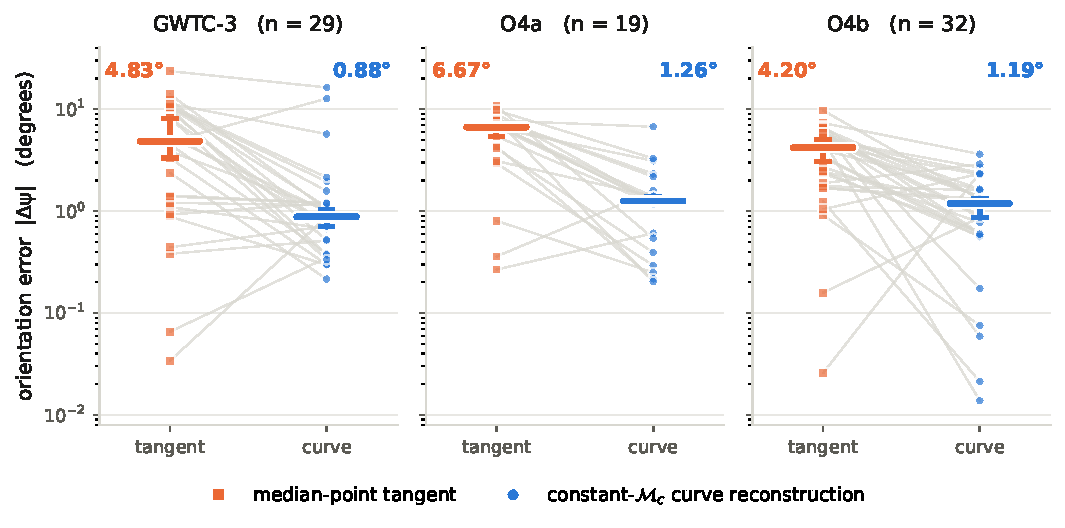
\includegraphics[width=0.86\textwidth]{../figures/fig1b_tangent_vs_curve_residual.pdf}
\caption{\figonebcaption}
\label{fig:1b}
\end{figure*}

\begin{figure*}[t]
\centering
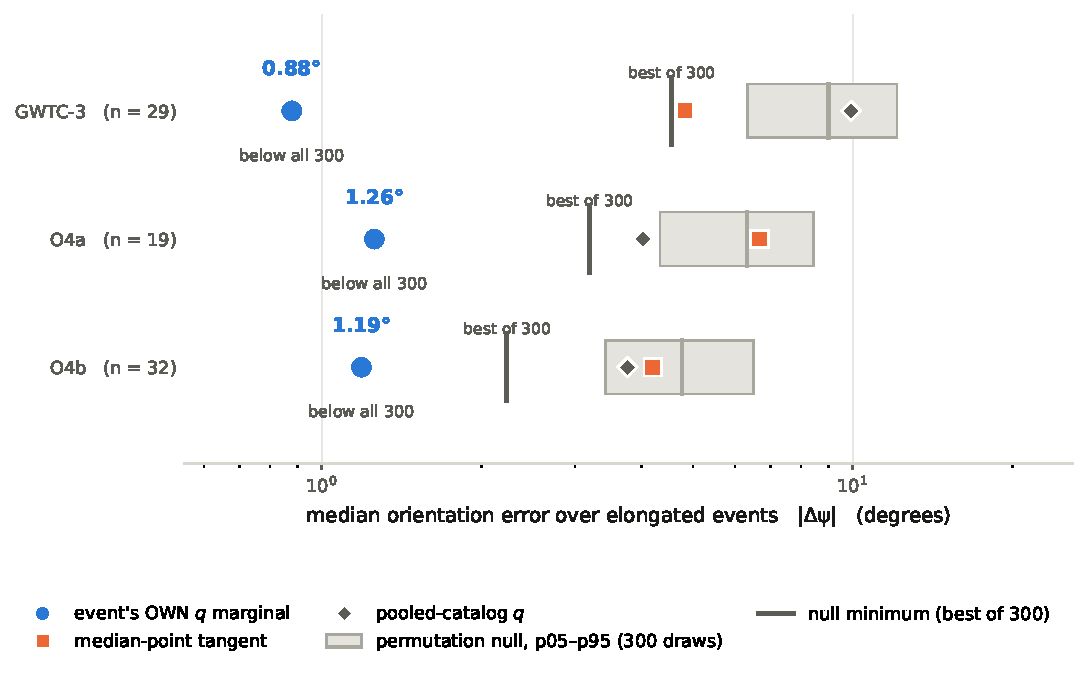
\includegraphics[width=0.80\textwidth]{../figures/fig1c_nontriviality_q_baselines.pdf}
\caption{\figoneccaption}
\label{fig:1c}
\end{figure*}

\subsection{The chirp-mass exponents carry the information}
\label{sec:nontrivial}
A curve describing a curved distribution better than a straight line is unsurprising, and a construction
with no free parameters cannot overfit. The substantive questions are whether the constant-$\mathcal{M}_c$
contour \emph{specifically} carries the information, and whether the \emph{event's own} marginal does.
Both hold.

First, the exponents matter. Generalising the contour to $m_1(q;p)\propto q^{-p}(1+q)^{2p-1}$, with
general relativity fixing $p=3/5$, and evaluating each alternative on the \emph{same} event's own
mass-ratio marginal, displacing the exponent to $p=0.50$ degrades the median orientation error to
$\AltErrObHalf$--$\AltErrOaHalf^\circ$, a factor of $\AltRatioMin$--$\AltRatioMax$ worse than the
general-relativistic value across the three catalogs. The error as a function of $p$ has a well-defined
minimum, at $p^\star=\AltPStarLo$--$\AltPStarHi$: slightly \emph{above} $3/5$. That small displacement
is real and physical, and Section~\ref{sec:onepn} shows it is the imprint of the next post-Newtonian
order rather than a defect of the construction.

The improvement over the local tangent is likewise not an artefact of an implausibly crude comparison. A
chord joining the contour at the 5th and 95th percentiles of the marginal --- a one-parameter stand-in for
the arc --- already improves substantially on the tangent, reaching $\ChordOa^\circ$ on O4a and
$\ChordOb^\circ$ on O4b; but the full arc improves on the chord by roughly a further factor of two, so the
curvature of the contour across the marginal carries information beyond its endpoints.

Second, the event's own marginal is required (Figure~\ref{fig:1c}): substituting any other event's does
not perform comparably.

Replacing the event's marginal with one pooled over the catalog, or with another event's, degrades the
median error by $\DegradeMin$--$\DegradeMax\times$. The band shown in Figure~\ref{fig:1c} is that null
distribution; it is not a confidence interval on the reconstruction. Under $\PermN$ catalog-stratified permutations of the
mass-ratio marginals among events, the achieved error lies below the \emph{minimum} of the null
distribution in every catalog, giving a permutation $p$-value $< 1/\PermN$ throughout. We report the full
permutation distribution rather than a single shuffled assignment because one draw is not a null: in O4a
the $\PermN$ draws span $\PermOaMin$--$\PermOaMax^\circ$, so any individual shuffle could have fallen
anywhere in that range.

\subsection{Transfer between waveform families}
\label{sec:xfam}
Because the mass-ratio marginal is taken from the posterior being reconstructed, a natural concern is
circularity: the agreement might reflect shared Monte Carlo noise rather than shared geometry. We test this
by crossing waveform families --- the \textsc{IMRPhenom} and \textsc{SEOBNR} analyses released for each
event (\texttt{IMRPhenomXPHM}/\texttt{SEOBNRv4PHM} in GWTC-3; \texttt{IMRPhenomXPHM-SpinTaylor}/%
\texttt{SEOBNRv5PHM} in O4a and O4b), with family~A the \textsc{IMRPhenom} member throughout. Using
family~A's mass-ratio marginal to predict family~B's independently
sampled principal axis --- never touching B's own geometry --- gives $\XfamAtoB^\circ$ (A$\to$B) and
$\XfamBtoA^\circ$ (B$\to$A) over $\XfamN$ events elongated in both, against tangent baselines of
$\XfamTanAtoB^\circ$ and $\XfamTanBtoA^\circ$ in the same directions. The reference scale is
$\XfamDisagree^\circ$, the median angle between the two families' own measured axes.

The reconstruction therefore transfers between separately sampled posteriors of the same event and is not
an artifact of reusing one posterior's Monte Carlo fluctuations. The test has a definite limit: the two
families analyse the same strain data with shared calibration and priors, so it excludes reuse of sampling
noise but not modelling error common to both. We describe $\XfamDisagree^\circ$ as a reference scale rather
than an error floor, since a reconstruction may in principle denoise a posterior functional and fall below
the raw disagreement between families.

\section{Origin of the residual}
\label{sec:residual}

\subsection{The residual exceeds the Monte Carlo resolution}
\label{sec:mcres}
The $\sim\!1^\circ$ residual is not sampling noise. Bootstrapping the released samples --- drawing one
index set and recomputing \emph{both} the measured axis and the prediction inputs from it, so that their
correlated Monte Carlo errors cancel --- gives a median resolution of $\ResidSigma^\circ$ on the
difference, against a median discrepancy of $\ResidMedian^\circ$. Because the bootstrap is computed per
event, the appropriate summary is the median of the per-event ratios, $\ResidRatio$; this is not the
ratio of the two medians just quoted, which is a different statistic. The
constant-$\mathcal{M}_c$ curve is an accurate but imperfect description of posterior orientation, and the
gap is a property of the model rather than of the sample count.

This bootstrap measures the Monte Carlo resolution of the released sample set, and is distinct from the
interval drawn in Figure~\ref{fig:1b}, which is a bootstrap over the event sample. It shrinks as more samples
are released and encodes nothing about detector noise, calibration, waveform systematics or population
variation; it is not a coverage statement, and we do not report the fraction of events falling within one
or two bootstrap widths as though it were.

The residual carries a signed component: the curve under-rotates relative to the measured axis by a median
$\SignedMedian^\circ$. This is not uniform across catalogs, being significant in the derivation catalog
($p\,\SignedPTrain$) and in O4a ($p=\SignedPOa$) but not in O4b ($p=\SignedPOb$), the newest and largest
of the three. We therefore report it per catalog.

\subsection{Failure of principal-curve self-consistency}
\label{sec:selfcons}
\citet{HastieStuetzle1989} define a principal curve by \emph{self-consistency}: $f(t) = \mathbb{E}[X \mid
t_f(X) = t]$, so that every point of the curve is the mean of the data projecting onto it. This is directly
testable for the constant-$\mathcal{M}_c$ curve, and it fails. Projecting each posterior sample onto its
nearest curve point and comparing that point with the mean of the samples landing there leaves a
perpendicular offset of about $\SelfViolation$ of the posterior's own scale: the constant-$\mathcal{M}_c$
curve is not a principal curve of the posterior.

The magnitude of that failure tracks the reconstruction residual. The per-event self-consistency violation
correlates with the per-event orientation residual at Spearman $\rho=\SelfRho$ ($p=\SelfP$) on the primary
projection grid, with $\rho$ between $\SelfRhoMin$ and $\SelfRhoMax$ across a sweep of grid resolutions, so
the result does not depend on that choice. Both quantities are measured rather than fitted, so the
correlation cannot be inflated by additional model freedom.

We describe this as tracking rather than explaining. Both quantities derive from the same posterior and the
same curve, so the correlation localises the residual within the geometry without establishing a mechanism,
and the corresponding correction does not survive out-of-sample. Replacing the curve by the conditional
means --- a single Hastie--Stuetzle iteration --- reduces the residual in sample, but the improvement is
grid-sensitive (median $\SelfIterMin$--$\SelfIterMax^\circ$ across the sweep) and in the cross-family test
it improves both directions while reaching $p<0.05$ in only one
($\SelfXfamAPure^\circ\!\to\!\SelfXfamACorr^\circ$, $p=\SelfXfamAP$;
$\SelfXfamBPure^\circ\!\to\!\SelfXfamBCorr^\circ$, $p=\SelfXfamBP$). We therefore do not present it as an
improved reconstruction.

\subsection{Finite posterior thickness}
\label{sec:thickness}
A second contributor is supported out-of-sample. The curve model has zero thickness, whereas a real
posterior has finite width perpendicular to the curve --- a median of $\ThickRelative$ of its total spread.
Learning that width profile on one waveform family and using it to predict another family's axis improves
on the zero-thickness curve in both directions ($\ThickAPure^\circ\!\to\!\ThickAMeas^\circ$,
$p=\ThickAP$; $\ThickBPure^\circ\!\to\!\ThickBMeas^\circ$, $p=\ThickBP$).

The \emph{arc-varying} part of that profile is not established: a constant thickness performs as well as
the measured profile in one direction, and simple linear or quadratic tapers match or exceed it in both. We
therefore attribute no specific fraction of the residual to the measured taper.

\subsection{A post-Newtonian origin for the exponent offset}
\label{sec:onepn}
The displacement of the best-fitting exponent slightly above $3/5$ (Section~\ref{sec:nontrivial}) has a
physical explanation that also bears on the residual. At leading (0PN) order the inspiral phase depends on
the masses only through $\mathcal{M}_c$, so the degenerate direction of the posterior is exactly the
constant-$\mathcal{M}_c$ contour. The next (1PN) term introduces a dependence on the symmetric mass ratio
$\eta$, which rotates that direction slightly and shifts the effective exponent above $3/5$.

We make this quantitative. Constructing the stationary-phase inspiral Fisher matrix in $(m_1,m_2)$ over the
inspiral band and taking its least-constrained direction --- using no information from the measured
posterior --- reproduces the constant-$\mathcal{M}_c$ tangent exactly at leading order (effective exponent
$0.600$), and at 1PN predicts an effective exponent of $\OnePNpeff$ (interquartile range
$\OnePNpeffLo$--$\OnePNpeffHi$). This parameter-free prediction matches the empirical optimum above and
the exponent fitted independently in Appendix~\ref{app:exponent} at the population level: the median
fitted exponent is $\AttrPStar$ against a median prediction of $\AttrPPred$, a difference consistent with
zero under a bootstrap over events.

The attribution has a precise boundary, and we state it. The fitted exponent declines with elongation even
after the 1PN prediction is partialled out (rank partial correlation $\AttrRhoPAax$, $p=\AttrRhoPAaxP$),
whereas the prediction itself carries no elongation dependence at all ($\rho=\AttrRhoPredAx$,
$p=\AttrRhoPredAxP$). Two mechanisms therefore coexist: the 1PN phasing sets the central displacement of
the exponent above $3/5$, and a distinct, elongation-dependent finite-width effect pulls the
most-elongated events back toward it. The 1PN term explains the offset of the population; it does not
explain its variation across events.

For reproducibility: the Fisher matrix uses the analytic Advanced-LIGO noise fit of Ajith (2011), the
band $[20\,\mathrm{Hz}, f_{\rm ISCO}]$ with $f_{\rm ISCO}=4397\,\mathrm{Hz}\,(M/M_\odot)^{-1}$, the
stationary-phase inspiral phase truncated at 1PN, spins set to zero, and central finite differences for
the mass gradients.

The rotation is a \emph{local} effect and accounts for only part of the residual: at the median point it
moves the predicted orientation from $\OnePNzero^\circ$ (leading order) to $\OnePNone^\circ$ (1PN), while
the full arc reaches $\sim\!1^\circ$. Most of the accuracy comes from integrating the curvature of the
contour across the marginal, not from the local direction; the remaining residual is shared between that
arc curvature and the finite posterior thickness of Section~\ref{sec:thickness}.

\section{Robustness}
\label{sec:robust}

\subsection{Frames and coordinates}
\label{sec:frames}
The measured quantity is a Euclidean principal-axis angle in fixed coordinates and is not
reparameterisation invariant. We state that dependence rather than assume it away. Repeating the primary
score in detector-frame masses gives $\FrameDetErr^\circ$ against $\FrameSourceErr^\circ$ in the source
frame, paired over the same $\FrameNPaired$ events ($p=\FramePairedP$); in $(\log m_1, \log m_2)$ it gives
$\FrameLogErr^\circ$. The log-mass improvement over the source frame is expected --- the curve is closer
to a straight line in logarithmic coordinates, so the zero-curvature part of the residual shrinks --- but
we retain the linear source frame as primary because it is the frame in which the construction was locked
and in which posteriors are reported. In $(\mathcal{M}_c, q)$ coordinates the construction is degenerate by design, since a
constant-$\mathcal{M}_c$ curve is a vertical line and the reconstruction carries no per-event content.

The detector-frame improvement is largely mediated by elongation rather than indicating a better-suited
model. Removing the redshift uncertainty that source-frame masses inherit makes posteriors markedly more
elongated (median axis ratio $\FrameAxrDet$ against $\FrameAxrSource$), and at matched axis ratio the two
frames no longer separate cleanly: in the $3$--$5$ band the detector frame is in fact worse
($\MatchedLowDet^\circ$ against $\MatchedLowSource^\circ$). The source frame remains the locked primary
score and the detector-frame comparison is post hoc.

\subsection{The elongation threshold}
\label{sec:gate}
The restriction to elongated posteriors is physical rather than tuned. As the covariance approaches
isotropy the principal axis ceases to be defined and the score degrades smoothly toward the random
baseline: the median error is $\BandRound^\circ$ for $\mathrm{axr}\in[1,1.5)$, then $\BandTwo^\circ$,
$\BandThree^\circ$, $\BandFour^\circ$ and $\BandFive^\circ$ for successive bands, approaching but never
reaching the $\RandomBaseline^\circ$ expected for a random angle modulo $180^\circ$. Nothing distinguishes
the chosen threshold of $3$: the error falls monotonically and smoothly across thresholds from $1.5$ to
$10$. Figure~\ref{fig:2a} illustrates the geometry for three events selected by stated rules, including the
worst case in the sample. That worst case (GW200308\_173609, $16^\circ$) is a high-mass system with an
irregular posterior --- precisely the regime where \citet{Baird2013} note that constant chirp mass stops
characterising the mass degeneracy cleanly, as anticipated in the limitations below. The reconstruction
does not always win: the local tangent achieves the smaller
error for $\TangentBeatsAll$ of elongated events, rising to $\TangentBeatsHigh$ above $\mathrm{axr}=8$,
where both approaches are already accurate and the arc correction is small. Any application relying on the
reconstruction should treat it as a typical rather than a guaranteed improvement.

\begin{figure*}[t]
\centering
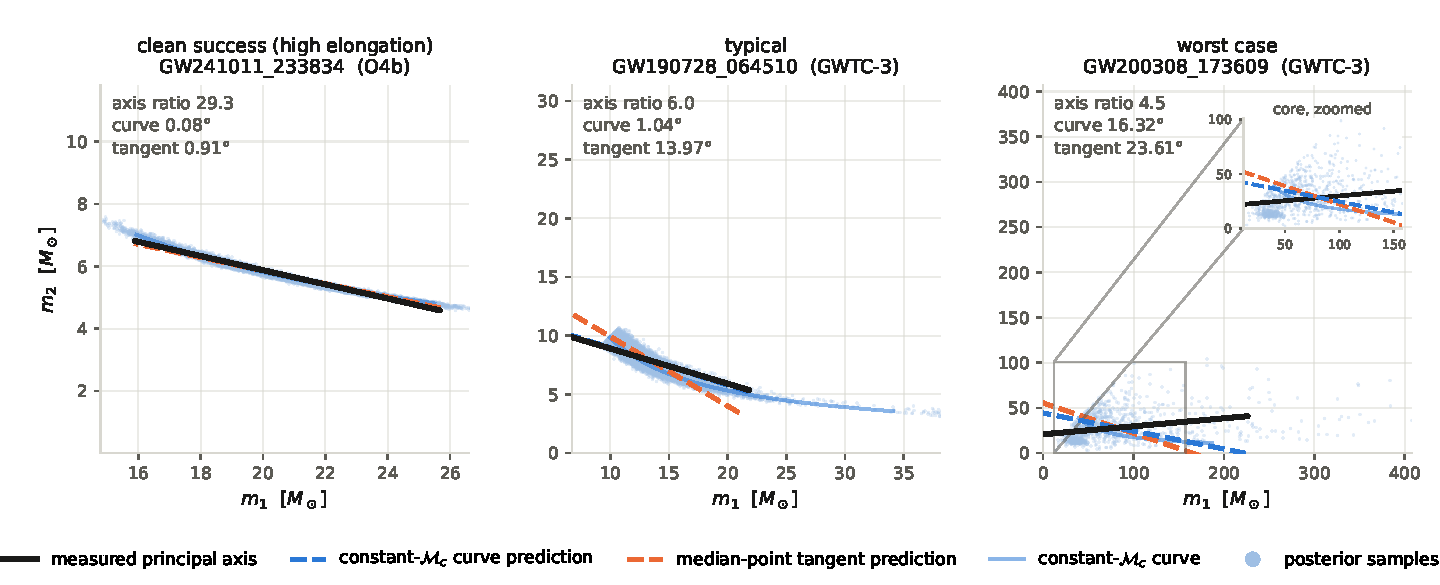
\includegraphics[width=0.72\textwidth]{../figures/fig2a_posterior_geometry_examples.pdf}
\caption{\figtwoacaption}
\label{fig:2a}
\end{figure*}

\subsection{Dependence on source parameters}
\label{sec:atlas}
If the geometry is measurement optics, the residual should not depend on source astrophysics. We test this
directly. Ranking the $\AtlasN$ elongated O4b events by their curve residual and correlating against nine
pre-declared axes --- precession $\chi_p$, aligned spin $\chi_{\rm eff}$, mass ratio, redshift,
signal-to-noise ratio, chirp mass, total mass, secondary mass, and waveform-family disagreement --- with
Benjamini--Hochberg control and a partial correlation removing the axis-ratio confound, no physical axis
survives. The only surviving correlate is waveform-model disagreement ($\rho=\AtlasWfRho$,
$q=\AtlasWfQ$), a measurement systematic. For this test, disagreement is the standard deviation of
$\psi_{\rm meas}$ across all waveform-family analyses of the event (mod-$180^\circ$ aligned), and the
residual is measured against the preferred family's axis. The correlation is \emph{negative}: events on
which the families disagree more show \emph{smaller} curve residuals. We do not have a derivation of this
sign --- a construction in which the curve tracked an ensemble consensus would naively predict the
opposite --- and we report it as an empirical association whose direction is unexplained.

This is a null result on $\AtlasN$ events and has correspondingly limited power. It bounds the size of any
physical dependence; it does not exclude one.

\section{Discussion}
\label{sec:discussion}
The orientation of a compact-binary mass posterior is reconstructible from a single one-dimensional
marginal of that posterior to about a degree on elongated events, with no coefficient calibrated on the
validation catalogs, and the reconstruction holds out-of-sample on two later, disjoint catalogs. It is not
the trivial observation that a curve outperforms a line: substituting another event's marginal degrades the
result several-fold, the achieved error lies below the minimum of $\PermN$ permutations, and the
reconstruction transfers between separately sampled waveform-family posteriors of the same event. The
residual is a systematic of the model, $\ResidRatio$ times the Monte Carlo resolution of the released
samples, to which finite posterior thickness is an out-of-sample contributor.

The tangent baseline quantifies what is being corrected. The principal axis of a Gaussian is the leading
eigenvector of its covariance, which for a likelihood expanded quadratically about its peak is the local
tangent to the degeneracy; the tangent error is therefore the error incurred by treating the posterior as
Gaussian. On elongated events that error is $\GaussTangentErr^\circ$ against $\GaussCurveErr^\circ$ once
the arc is accounted for --- a factor of $\GaussRatio$. The correction is essentially free, requiring only
the mass-ratio marginal that parameter estimation already produces, and its downstream effect is specific
rather than universal. It does not improve the total credible-region \emph{coverage} of a Gaussian
single-event approximation, which is set by the region's area and is nearly insensitive to its tilt (the
$90\%$ region captures $\DownCovTangent$ of the true posterior when tangent-oriented, against
$\DownCovOracle$ for the true axis). It does improve the component-mass \emph{marginals}, which are
orientation-sensitive: a tangent-oriented Gaussian misstates the secondary-mass $90\%$ credible width by a
median $\DownSecTangent$, which the arc reduces to $\DownSecCurve$, close to the $\DownSecOracle$ of the true
axis. (These Gaussians are moment-matched --- true sample mean and covariance eigenvalues, orientation
set as stated --- and the figures are medians over the $\ResidNElong$ elongated events.) Any analysis
that reads component-mass intervals from a Gaussian single-event approximation therefore benefits; the
clearest existing consumer is low-latency source classification, which thresholds on the secondary mass
to distinguish binary classes. A template-placement or volume estimate that uses only the metric area
does not benefit.

\paragraph{Scope.} Three boundaries are worth stating together, since each has a natural stronger reading
that the measurements do not support. First, the relation uses a marginal of the posterior it
reconstructs, not information external to it: the mass-ratio marginal is drawn from that same posterior.
Both the input marginal and the target covariance inherit the sampling priors of the released analyses, so
the geometry characterised here is that of the likelihood--prior product, not of the likelihood alone; for
quiet events, where the mass-ratio marginal is substantially prior-driven, the diagnostic's meaning shifts
with the prior choice, and we have not quantified that dependence.
Second, the reconstructed quantity is a Euclidean angle in fixed coordinates, and Section~\ref{sec:frames}
shows it changes with the choice of mass variables; we therefore report the convention rather than claim
invariance, and do not appeal to {\v C}encov's uniqueness theorem for the Fisher--Rao metric, which would
assert the opposite of what we measure. Third, we use the stiff/sloppy vocabulary
\citep{Transtrum2015} for the concept only. The stronger ``hyperribbon'' picture, in which the covariance
eigenvalue spectrum spans many orders of magnitude, does not follow from these data: in the
two-dimensional mass plane the eigenvalue ratio has a median of $\EigRatioMedian$, with $\EigFracDecade$
of events exceeding one order of magnitude and $\EigFracTwoDec$ exceeding two. Sloppiness in that sense is
a property of the full parameter space, which a two-dimensional marginal cannot establish.

The posteriors analysed here were generated with general-relativistic waveform models, so structure found
in their geometry probes the internal consistency of those inferences rather than the theory that produced
them, and no bound on modified inspiral phasing follows. Appendix~\ref{app:exponent} develops this
quantitatively for a one-parameter generalisation of the chirp-mass exponents, where a naive reading gives
an apparent $\ExpNaiveSigma\sigma$ departure from the general-relativistic value that two pre-committed
checks reduce to $\ExpSigma\sigma$.

\paragraph{Limitations.} We record the following, roughly in order of how much they constrain use of the
result.
\begin{enumerate}\itemsep2pt \parskip0pt
\item Waveform-model choice contributes a per-event orientation scatter of several degrees and is the
dominant per-event systematic.
\item The relation is validated on elongated posteriors. Round posteriors have no well-defined orientation
and are excluded by construction, and \citet{Baird2013} note that constant chirp mass characterises the
mass degeneracy less cleanly at higher masses, bounding where the construction should be expected to hold.
\item O4a and O4b are disjoint event catalogs, not independent experiments: they share detectors,
calibration, waveform families, priors and analysis conventions.
\item The two out-of-sample scores are not equal evidence. The O4b registration is timestamped in the
public record before the data were opened; the O4a registration entered the public repository in the same
commit as its results and is attested only by a private history.
\item The residual is tracked by the curve's failure of self-consistency, but the corresponding one-step
correction does not survive out-of-sample, and the arc-varying form of the thickness contribution is not
established.
\item A first-principles derivation of the curve's width and curvature from the Fisher information remains
open.
\end{enumerate}

\section{Conclusions}
\label{sec:conclusions}
The orientation of the component-mass posterior of a compact binary is not merely qualitatively aligned
with a constant-chirp-mass contour but quantitatively reconstructible from the event's mass-ratio marginal,
to a median $\LockedOaCurveElong^\circ$ and $\LockedObCurveElong^\circ$ on two catalogs released after the
prediction was fixed. The reconstruction requires the event's own marginal, transfers between waveform
families, and leaves a residual that is a property of the model rather than of finite sampling.

Two consequences follow. First, the local Gaussian approximation underlying rapid parameter-estimation
tools misstates posterior orientation by a factor of $\GaussRatio$ more than the arc-corrected
construction. This is a cheap correction with a specific benefit: it reduces the error in the
component-mass credible intervals of a Gaussian single-event approximation from a median $\DownSecTangent$
to $\DownSecCurve$ on the secondary mass, while leaving the total credible-region coverage --- which does
not depend on orientation --- unchanged. Second,
because the geometry is this reproducible, departures from it are measurable, and we find no dependence on
any of nine pre-declared source parameters --- the only surviving correlate is waveform-model disagreement.
A first-principles derivation of the curve's thickness and curvature from the Fisher information, and a
strain-level rather than model-level test of the underlying information geometry, remain open.

\appendix

\section{A geometric exponent diagnostic}
\label{app:exponent}
The exponents in Eq.~(\ref{eq:curve}) are fixed by the leading-order quadrupole formula. Generalising to a
one-parameter family,
\begin{equation}
\mathcal{M}_p = (m_1 m_2)^p (m_1+m_2)^{1-2p},
\end{equation}
with $p = 3/5 = 0.600$ in general relativity. Fitting $p$ to the posterior orientations isolates the exponent from the mass scale, since orientation
is scale-free ($m_1(q;p) \propto q^{-p}(1+q)^{2p-1}$).

On the O4b elongated events we find $p = \ExpOb \pm \ExpObErr$; combining O4a and O4b gives
$p = \ExpComb \pm \ExpCombErr$, formally $\ExpNaiveSigma\sigma$ from $p=3/5$. This is not a deviation
from general relativity, and it is not a statistical fluctuation to be explained away: it is the imprint
of the next post-Newtonian order, predicted from first principles in Section~\ref{sec:onepn}. The 1PN
$\eta$-dependent phasing shifts the effective degeneracy exponent to $\OnePNpeff$, in agreement with the
fitted value here and with the empirical optimum of Section~\ref{sec:nontrivial}.

Two further properties bound the offset, and both were pre-committed. The two disjoint catalogs disagree
with each other by $\ExpSpread$, comparable to the offset from the general-relativistic value
($\ExpOffset$), so the catalog-to-catalog spread is a systematic that the bootstrap statistical error
($\ExpCombErr$) does not capture; including it gives $\ExpSigma\sigma$. And the per-event exponent
depends on elongation (Spearman rank correlation $\rho = \ExpSpearman$ over the elongated events of both
catalogs), with the most-elongated half yielding $p=\ExpCleanHalf$. As Section~\ref{sec:onepn} shows
quantitatively, this elongation dependence is \emph{not} carried by the 1PN prediction, which is flat in
axis ratio: the 1PN phasing sets the central displacement, and a distinct finite-width effect produces the
variation with elongation. The combined value quoted above weights the two catalogs by inverse variance.
No bound on modified inspiral phasing follows from any of this, and we draw none: the posteriors were
generated with general-relativistic waveforms.

\section{Reproducibility}
\label{app:repro}
All analyses read a single cached extract of the released posterior samples, so that every downstream
result shares one deterministic input and can be regenerated without re-reading the parameter-estimation
files. The extract performs no subsampling: it stores every sample passing the finiteness and mass-ratio
cuts, $\CacheSamples$ million samples across $\CacheRows$ waveform-group rows, with $\CacheRowsExact$ of
those $\CacheRows$ rows held in full. A cache-backed number is therefore a full-sample number and carries
no resampling noise.

As a consistency check, an independent pass that re-reads the released files directly, bypassing the cache,
returns $\FullOaCurve^\circ$ for O4a and $\FullObCurve^\circ$ for O4b, against $\CacheOaCurve^\circ$ and
$\CacheObCurve^\circ$ from the cache. For the derivation catalog the two differ by $0.08^\circ$, because
they resolve one event's preferred waveform group differently; this is a selection convention rather than
a sampling effect.

Every number in this paper --- in the abstract, the text, Table~\ref{tab:curve} and every figure caption
--- is emitted from a committed machine-readable artifact and inserted into the manuscript source as a
generated macro rather than typed, so that text, table and figure cannot drift from the analysis or from
one another. Figure captions are generated from the same sidecar files that produce the figures.

\section*{Data availability}
This work is a reanalysis of public parameter-estimation data. It uses no proprietary or embargoed
products and generates no new observational data. Three releases are used, obtained from the Gravitational
Wave Open Science Center (GWOSC) \citep{GWOSCthree} and Zenodo: GWTC-2.1 \citep{GWTC21} and GWTC-3
\citep{GWTC3} posterior samples; the GWTC-4.0/O4a release \citep{GWTC4}, Zenodo record 16053484; and the
GWTC-5.0/O4b release \citep{GWTC5}, Zenodo records 20276106 and 20348006. GWOSC data are distributed under
a Creative Commons Attribution licence and are used here under those terms. Analysis code, registered
predictions, per-event results and the figure-generation pipeline accompany this work; record numbers and
download procedures are given in the accompanying data-availability documentation.

\section*{Acknowledgments}
This research has made use of data or software obtained from the
Gravitational Wave Open Science Center (gwosc.org), a service of the LIGO Scientific Collaboration, the
Virgo Collaboration, and KAGRA
\citep{GWOSCthree,GWOSCfourA,GWOSCfourB}. LIGO is funded by the U.S. National Science Foundation. Virgo is
supported through the European Gravitational Observatory (EGO), by the French Centre National de Recherche
Scientifique (CNRS), the Italian Istituto Nazionale di Fisica Nucleare (INFN) and the Dutch Nikhef, with
contributions by institutions from Belgium, Germany, Greece, Hungary, Ireland, Japan, Monaco, Poland,
Portugal and Spain. KAGRA is supported by the Ministry of Education, Culture, Sports, Science and
Technology (MEXT) and the Japan Society for the Promotion of Science (JSPS) in Japan; the National Research
Foundation (NRF) and the Ministry of Science and ICT (MSIT) in Korea; and Academia Sinica (AS) and the
National Science and Technology Council (NSTC) in Taiwan.

This is independent work carried out entirely on public data. The author is not a member of the
LIGO--Virgo--KAGRA Collaboration; the Collaboration has not reviewed this
analysis and bears no responsibility for its conclusions.

\paragraph{Use of AI assistants.} Large language models were used in this work and are disclosed here
in the form journal policy now requires. \emph{Tools:} Anthropic's Claude (Opus 4.8, via Claude Code) and
OpenAI's Codex. \emph{How they assisted:} Claude implemented the analysis code and the figure and
number-generation pipelines and drafted the manuscript; Codex performed independent adversarial review of
both the analysis and the text over repeated rounds. \emph{How they were directed:} by the author, through
task-level instructions specifying the measurement to be made, the preregistered decision rules to be
respected, and the artifacts against which each claim was to be checked; neither model had discretion over
what was claimed or which results were reported. \emph{How output was verified:} every number in this
paper is regenerated from a committed machine-readable artifact rather than transcribed
(Appendix~\ref{app:repro}), a contract test suite fails if manuscript and artifacts disagree, and the
author reviewed each result before inclusion. The author defined the research questions, registered every
preregistered decision before the corresponding data were examined, and is
solely responsible for the content of this paper. The models are tools, not authors.

The author thanks the Collaboration for releasing the
parameter-estimation samples on which the analysis wholly depends, and the open-source scientific Python
community for NumPy \citep{numpy}, SciPy \citep{scipy}, Matplotlib \citep{matplotlib} and h5py.

\begin{thebibliography}{99}
\bibitem[Cutler \& Flanagan(1994)]{CutlerFlanagan1994} C.~Cutler and {\'E}.~{\'E}.~Flanagan,
\emph{Phys.\ Rev.\ D} \textbf{49}, 2658 (1994).
\bibitem[Poisson \& Will(1995)]{PoissonWill1995} E.~Poisson and C.~M.~Will,
\emph{Phys.\ Rev.\ D} \textbf{52}, 848 (1995).
\bibitem[Baird et al.(2013)]{Baird2013} E.~Baird, S.~Fairhurst, M.~Hannam, and P.~Murphy,
\emph{Phys.\ Rev.\ D} \textbf{87}, 024035 (2013).
\bibitem[Hannam et al.(2013)]{Hannam2013} M.~Hannam, D.~A.~Brown, S.~Fairhurst, C.~L.~Fryer, and
I.~W.~Harry, \emph{Astrophys.\ J.\ Lett.} \textbf{766}, L14 (2013).
\bibitem[Ohme et al.(2013)]{Ohme2013} F.~Ohme, A.~B.~Nielsen, D.~Keppel, and A.~Lundgren,
\emph{Phys.\ Rev.\ D} \textbf{88}, 042002 (2013).
\bibitem[Fairhurst et al.(2023)]{Fairhurst2023} S.~Fairhurst, C.~Hoy, R.~Green, C.~Mills, and
S.~A.~Usman, \emph{Phys.\ Rev.\ D} \textbf{108}, 082006 (2023).
\bibitem[Makinen et al.(2026)]{Makinen2026} T.~L.~Makinen, D.~J.~Bartlett, N.~Jeffrey, and
B.~D.~Wandelt, \emph{The Degeneracy Distillery}, arXiv:2606.23838 (2026).
\bibitem[Transtrum et al.(2015)]{Transtrum2015} M.~K.~Transtrum et al.,
\emph{J.\ Chem.\ Phys.} \textbf{143}, 010901 (2015).
\bibitem[Hastie \& Stuetzle(1989)]{HastieStuetzle1989} T.~Hastie and W.~Stuetzle,
\emph{J.\ Amer.\ Statist.\ Assoc.} \textbf{84}, 502 (1989).
\bibitem[LVK(2025)]{GWTC4} The LIGO Scientific, Virgo and KAGRA Collaborations,
\emph{GWTC-4.0: Updating the Gravitational-Wave Transient Catalog with Observations from the First Part
of the Fourth LIGO--Virgo--KAGRA Observing Run}, arXiv:2508.18082 (2025).
\bibitem[LVK(2026c)]{GWTC5} The LIGO Scientific, Virgo and KAGRA Collaborations,
\emph{GWTC-5.0: Observations from the Second Part of the Fourth LIGO--Virgo--KAGRA Observing Run and
Updates to the Gravitational-Wave Transient Catalog}, arXiv:2605.27225 (2026).
\bibitem[LVK(2023)]{GWOSCthree} R.~Abbott et al. (KAGRA, LIGO Scientific and Virgo Collaborations),
\emph{Astrophys.\ J.\ Suppl.\ Ser.} \textbf{267}, 29 (2023), arXiv:2302.03676.
\bibitem[LVK(2026a)]{GWOSCfourA} The LIGO Scientific, Virgo and KAGRA Collaborations,
\emph{Open Data from LIGO, Virgo, and KAGRA through the First Part of the Fourth Observing Run},
\emph{Astrophys.\ J.} \textbf{1004}, 2329 (2026).
\bibitem[LVK(2026b)]{GWOSCfourB} The LIGO Scientific, Virgo and KAGRA Collaborations,
\emph{Open Data from LIGO, Virgo, and KAGRA through the Second Part of the Fourth Observing Run},
arXiv:2605.27090 (2026).
\bibitem[LVK(2024)]{GWTC21} R.~Abbott et al. (LIGO Scientific and Virgo Collaborations),
\emph{Phys.\ Rev.\ D} \textbf{109}, 022001 (2024), arXiv:2108.01045.
\bibitem[LVK(2023b)]{GWTC3} R.~Abbott et al. (LIGO Scientific, Virgo and KAGRA Collaborations),
\emph{Phys.\ Rev.\ X} \textbf{13}, 041039 (2023), arXiv:2111.03606.
\bibitem[Harris et al.(2020)]{numpy} C.~R.~Harris et al., \emph{Nature} \textbf{585}, 357 (2020).
\bibitem[Virtanen et al.(2020)]{scipy} P.~Virtanen et al., \emph{Nat.\ Methods} \textbf{17}, 261 (2020).
\bibitem[Hunter(2007)]{matplotlib} J.~D.~Hunter, \emph{Comput.\ Sci.\ Eng.} \textbf{9}, 90 (2007).
\end{thebibliography}

\end{document}
